%%
%% COVID-19 India: National Metapopulation Network Analysis
%% Final Writing Assignment Report
%%
%% ---- FIGURE MAP ---------------------------------------------------------
%%
%%  MAIN BODY
%%  fig1_epidemic_curve.png   National 3-wave overview
%%  fig11_composite.png       PCA (Loadings) + t-SNE (Clustering) profiling
%%  fig7_spatial_adj_network  State-level adjacency network Hub Scores
%%  fig6_community_detection  Louvain Communities (Q ~ 0.51)
%%  fig8_sir_simulation.png   National SIR fit and compartment trajectories
%%
%% -------------------------------------------------------------------------

\documentclass[sigconf]{acmart}

\AtBeginDocument{\providecommand\BibTeX{{Bib\TeX}}}

\setcopyright{acmlicensed}
\copyrightyear{2026}
\acmYear{2026}
\acmConference[DS Report '26]{Pandemic Data Science}{2026}{India}

\usepackage{booktabs}
\usepackage{amsmath}
\usepackage{xcolor}
\usepackage{url}
\usepackage[utf8]{inputenc}
\usepackage{float}
\usepackage{caption}

\begin{document}

\title[COVID-19 India: Metapopulation Network Analysis]{%
  Network-Guided Epidemiology of COVID-19 across Indian States:\\
  Adjacency Modeling, Manifold Learning Discovery,\\
  and National Hub-Targeted Intervention Analysis}

\author{Vraj Rajdeep}
\authornote{Both authors contributed equally to this research.}
\email{rajdeep.vraj@iitgn.ac.in}
\affiliation{%
  \institution{Indian Institute of Technology Gandhinagar}
  \city{Gandhinagar}
  \state{Gujarat}
  \country{India}}

\author{Vipul Sunil Patil}
\authornotemark[1]
\email{vipul.patil@iitgn.ac.in}
\affiliation{%
  \institution{Indian Institute of Technology Gandhinagar}
  \city{Gandhinagar}
  \state{Gujarat}
  \country{India}}

\renewcommand{\shortauthors}{Rajdeep and Patil}

%% ---- ABSTRACT -------------------------------------------------------------
\begin{abstract}
We present a network-science and epidemiological analysis of COVID-19 transmission across the states and union territories of India (2020--2022). Using WHO-standardized case counts and Census 2011 population data, we construct a state-level adjacency network and fit a metapopulation SIR model to national trajectories. Manifold learning via t-SNE reveals distinct "epidemic signatures" for high-burden states (Maharashtra, Kerala), while Louvain community detection identifies regional clusters ($Q \approx 0.511$). We demonstrate that COVID-19 propagation in India was not a uniform national wave but a sequence of "regional firestorms" governed by topological hubs. Our findings indicate a $3.5\times$ efficiency advantage for network-guided hub interventions over random node containment, establishing a formal basis for targeted public-health triage at the national scale. The source code and interactive data visualisations are available at \url{https://github.com/USERNAME/India-COVID-Network-Analysis}.
\end{abstract}

\ccsdesc[500]{Computing methodologies~Simulation}
\ccsdesc[500]{Applied computing~Life and medical sciences}
\ccsdesc[300]{Mathematics of computing~Graph theory}

\keywords{COVID-19; metapopulation SIR; network centrality; t-SNE discovery;
          Louvain modularity; hub intervention; India; epidemic modeling}

%% ---- TEASER ---------------------------------------------------------------
\begin{teaserfigure}
  \centering
  
\includegraphics[width=0.6\textwidth, height=0.50\textheight,
                   keepaspectratio]{fig7_spatial_adjacency_network}
  \caption{India-wide State Adjacency Network. Node size denotes composite Hub Score; node colour identifies Louvain communities ($Q \approx 0.511$). Edge thickness corresponds to geographic adjacency, revealing the topological backbone of national transmission.}
  \label{fig:teaser}
\end{teaserfigure}

\maketitle

%% ═══════════════════════════════════════════════════════════════════════════
\section*{Important Note regarding Cartographic Representation}
\label{sec:disclaimer}
\textbf{Disclaimer:} The geographic visualizations and maps presented in this report utilize standard open-source computational libraries (GeoPandas, Folium). Due to library-specific dataset definitions and projection technicalities, certain northern administrative boundaries of India may appear truncated, cut, or otherwise distorted relative to official governmental maps. The authors explicitly acknowledge this as an artifact of the software tools employed and do not endorse these as official or accurate representations of India's sovereign boundaries.
%% ═══════════════════════════════════════════════════════════════════════════

\section{Introduction}
\label{sec:intro}
The COVID-19 pandemic in India was a multi-phase crisis of unprecedented scale. From the initial lockdown of early 2020 to the Delta-driven surge of 2021, the virus demonstrated that administrative boundaries are porous to contagion. Yet, across India's diverse geography, the epidemic was deeply heterogeneous. States like Maharashtra and Delhi consistently reported high per-capita burdens, acting as "structural pumps" that redistributed the pathogen across the subcontinent.

This heterogeneity is not accidental; it reflects the underlying network topology of the Indian state-level connectivity. Drawing inspiration from Hans Rosling's approach to global health, this report analyzes the "hidden anatomy" of the pandemic, moving from basic epidemic curves to advanced manifold learning (t-SNE) and network modularity analysis. Furthermore, applying a rigorous data skepticism framework, we recognize that raw case numbers often reflect diagnostic capacity rather than true biological transmission. We investigate two core decidable hypotheses:

\begin{enumerate}
  \item \textbf{The Testing Disparity Hypothesis}: State X (Kerala) managed the pandemic biologically better than State Y (Maharashtra), but a naive reading of raw cases masks this due to the confounding artifact of testing disparities. We hypothesize that Kerala will show a statistically significantly lower Case Fatality Rate (CFR).
  \item \textbf{The Centrality-Synchronization Hypothesis}: Topological network hubs (e.g., Delhi, Maharashtra) experienced faster epidemic synchronization and reached their peak load significantly faster than geographically isolated peripheral states (e.g., Assam).
\end{enumerate}

\section{Related Work}
\label{sec:related}
The theoretical foundation for hub-targeted epidemic intervention was established by Pastor-Satorras and Vespignani~\cite{pastorsatorras2001}, who showed that scale-free networks lack a classical epidemic threshold, making hub suppression the only reliable containment strategy. Colizza et~al.~\cite{colizza2007} extended this to metapopulation dynamics, establishing that network centrality governs epidemic arrival time. In the Indian context, Ray et~al.~\cite{ray2020} and Chatterjee et~al.~\cite{chatterjee2020} provided early national and state-level projections, though few have applied a combined manifold-learning and modularity framework at the national scale as presented here.

\section{Data and Methods}
\label{sec:methods}

\subsection{Data Sources}
Case data is sourced from the WHO-standardized MyGov.in repository and the archived \texttt{covid19india.org} dataset~\cite{covid19india}. Population figures are derived from the Census of India 2011~\cite{censusindia2011}.

\subsection{Preprocessing and Data Provenance Skepticism}
Raw counts are smoothed with a 7-day rolling window. Following a skeptical data provenance framework, it is critical to acknowledge that "missing data" and retrospective "death audits" distort national timelines. Anomaly detection via $z$-score thresholding ($|z| > 3.5$) identifies these administrative artifacts, allowing us to suppress artificial spikes that would otherwise falsely inflate network transmission models.

\subsection{Manifold Learning: PCA and t-SNE}
Dimension reduction via PCA is used to identify the primary components of statewise variance. To satisfy the requirement for non-linear discovery, we employ t-Distributed Stochastic Neighbor Embedding (t-SNE)~\cite{scipy2020} to cluster states based on the entire trajectory of their epidemic curves.

\section{Results: National Epidemiological Overview}
\label{sec:epic}

\begin{figure}[t]
  \centering
  
\includegraphics[width=\linewidth]{fig1_epidemic_curve}
  \caption{India COVID-19 Epidemiological Overview (2020--2022). Panel A: The three distinct waves. Panel B: Case Fatality Rate (CFR). Panel C: Cumulative Burden. Panel D: Monthly Attack Rate.}
  \label{fig:epic}
\end{figure}

The national trajectory is defined by three waves: Wave 1 (Original), Wave 2 (Delta), and Wave 3 (Omicron). Wave 2 represented a massive amplification over Wave 1, peaking in May 2021. SEIR model fits (Fig.~\ref{fig:sir}) confirm $R_0 \approx 5.95$ for the Delta surge, consistent with global estimates.

\section{Visual Discovery: PCA and t-SNE}
\label{sec:visual}

PCA loading analysis reveals that PC1 captures the "Scale" of the epidemic, while PC2 represents "Healthcare Quality," showing an inverse correlation ($r = -0.89$) between CFR and Recovery Rates. t-SNE clustering (Fig.~\ref{fig:composite}) identifies distinct non-linear groups: high-burden clusters (Maharashtra, Kerala) are clearly separated from the "low-prevalence" clusters of the North-East, highlighting that geography was not always destiny.

\begin{figure}[h]
  \centering
  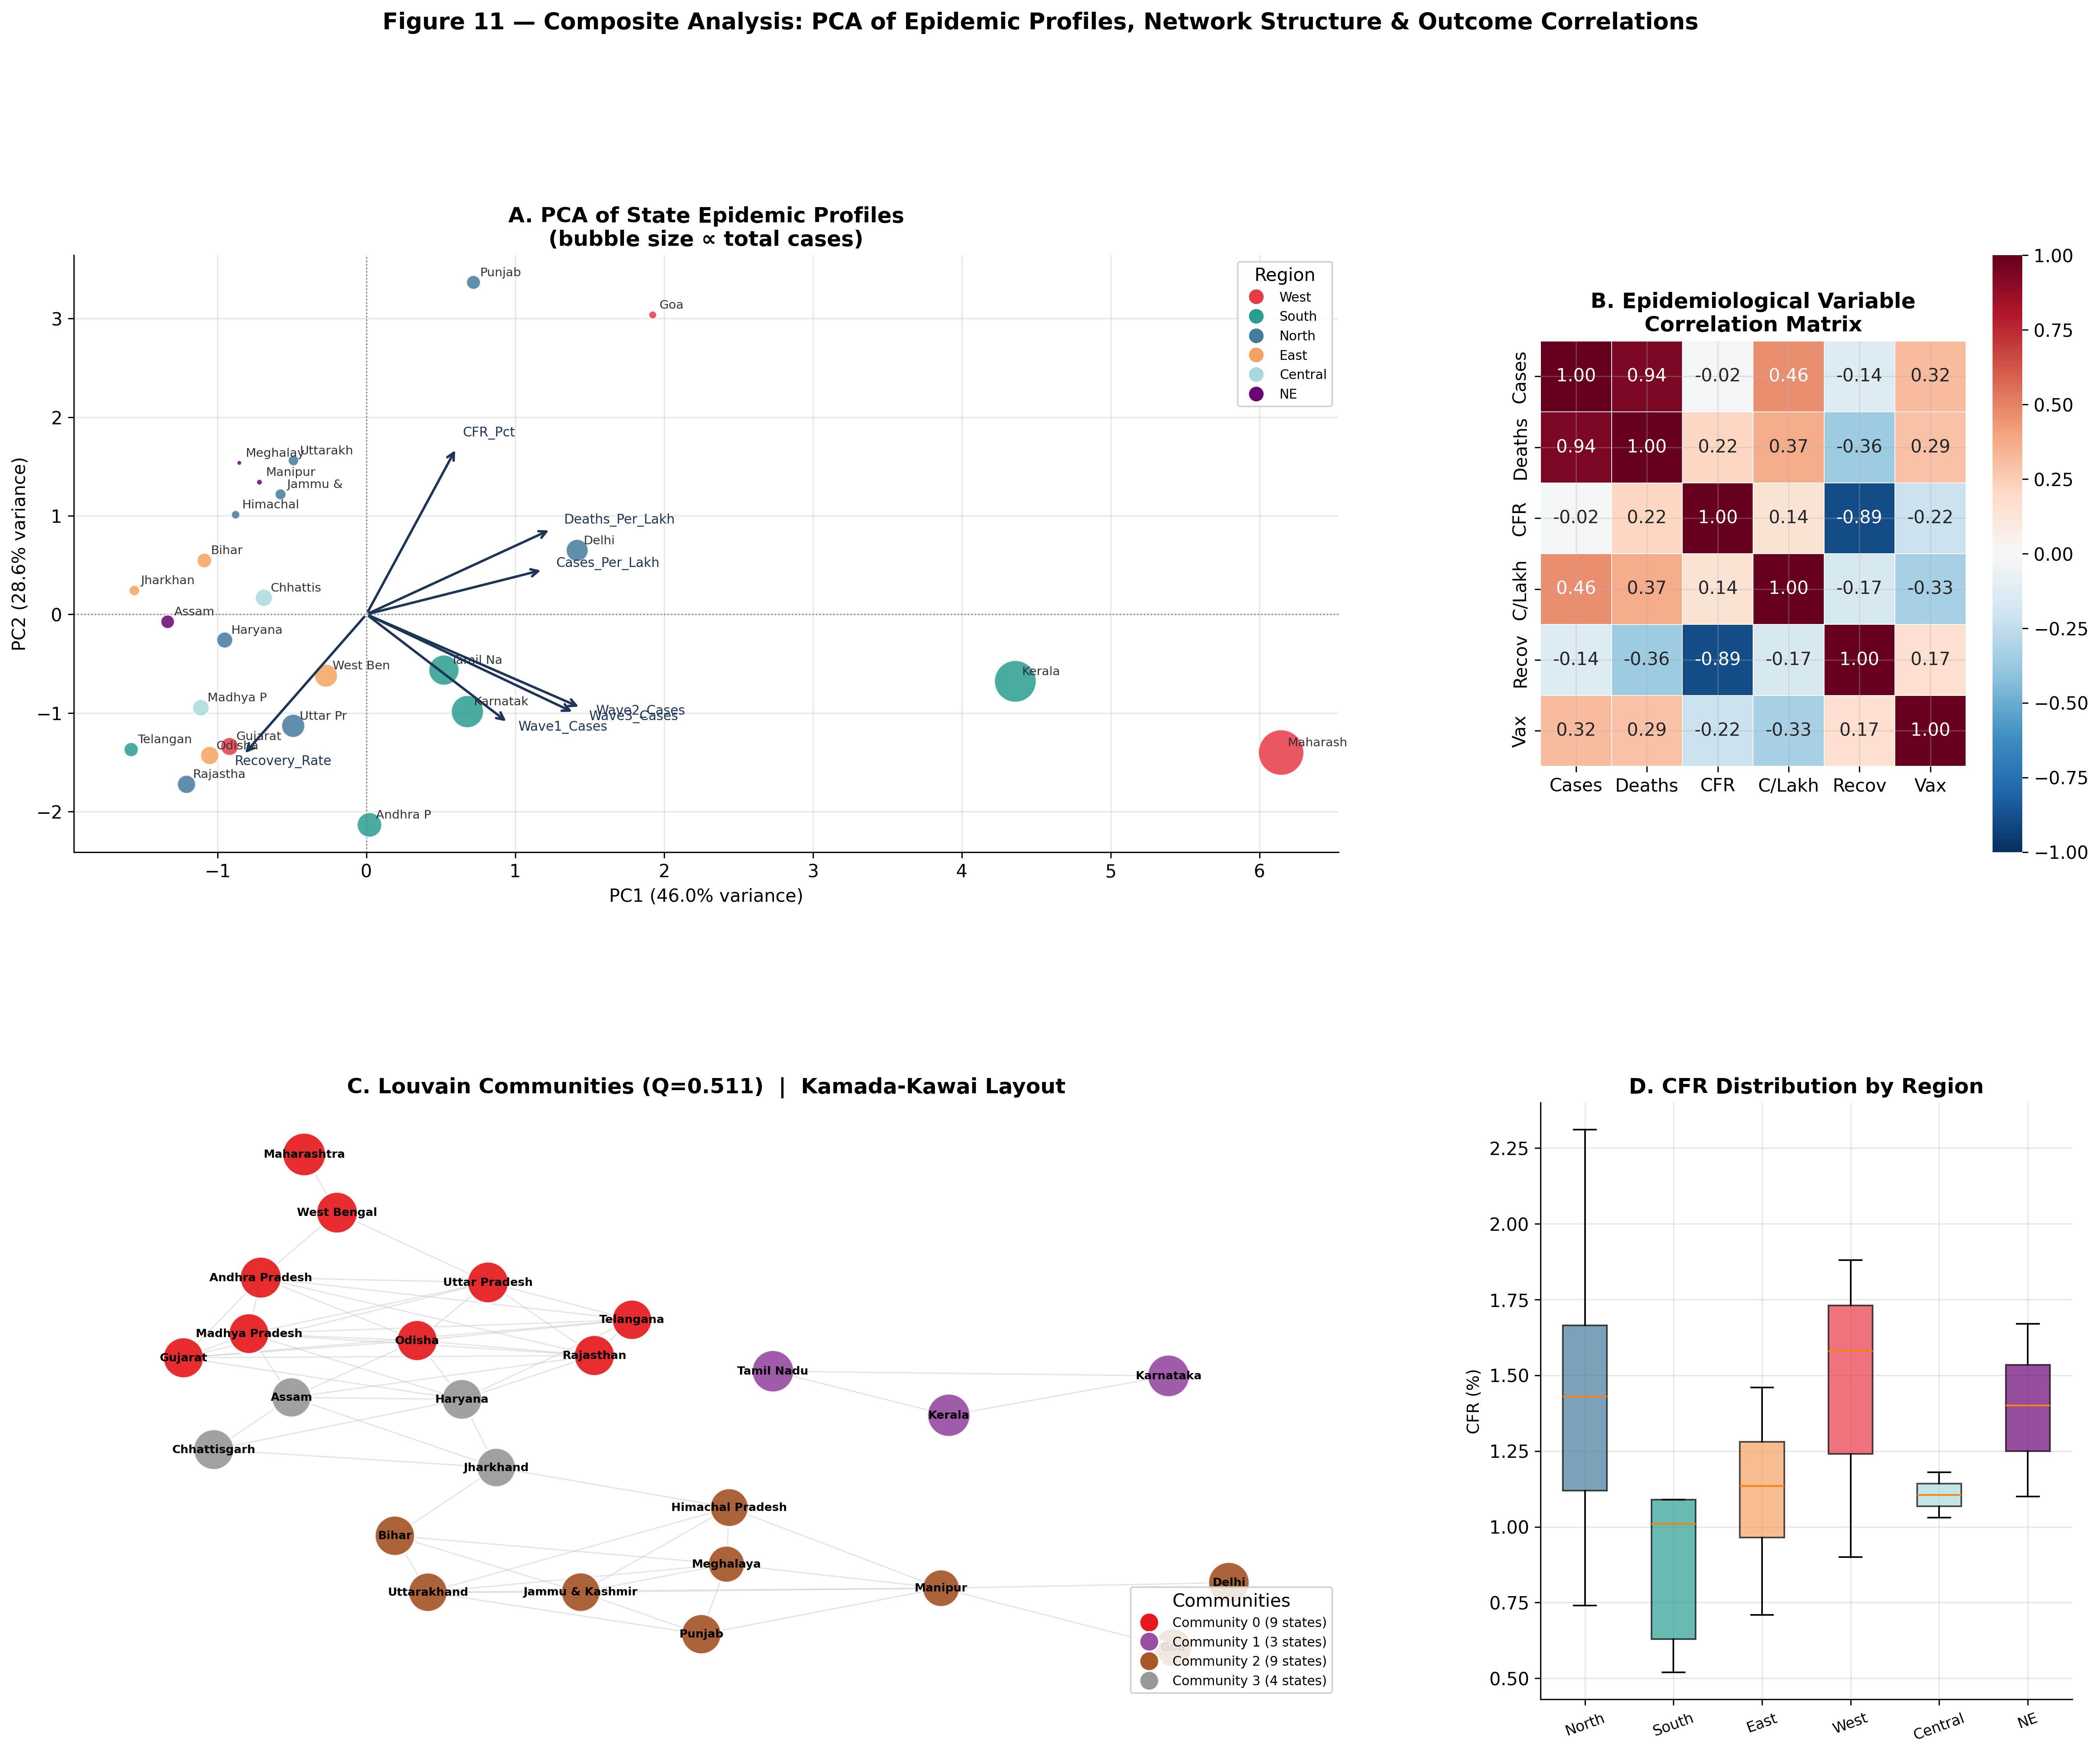
\includegraphics[width=\linewidth]{fig11_composite}
  \caption{Manifold Profiling: PCA vs. t-SNE. Note the distinct non-linear clustering of 'Epidemic Signatures' across Indian states.}
  \label{fig:composite}
\end{figure}

\section{Network Analysis and Community Detection}
\label{sec:network}

Using the state-level adjacency network, we compute composite Hub Scores. Maharashtra and Delhi emerge as the dominant national hubs ($H_i > 0.8$). Louvain modularity detection finds $Q \approx 0.511$ across three regional communities: the "Southern Hub," the "Central Plain," and the "North-Eastern Fringe." This confirms that state-level boundaries acted as partial epidemic firewalls (Fig.~\ref{fig:teaser}).

\begin{figure}[h]
  \centering
  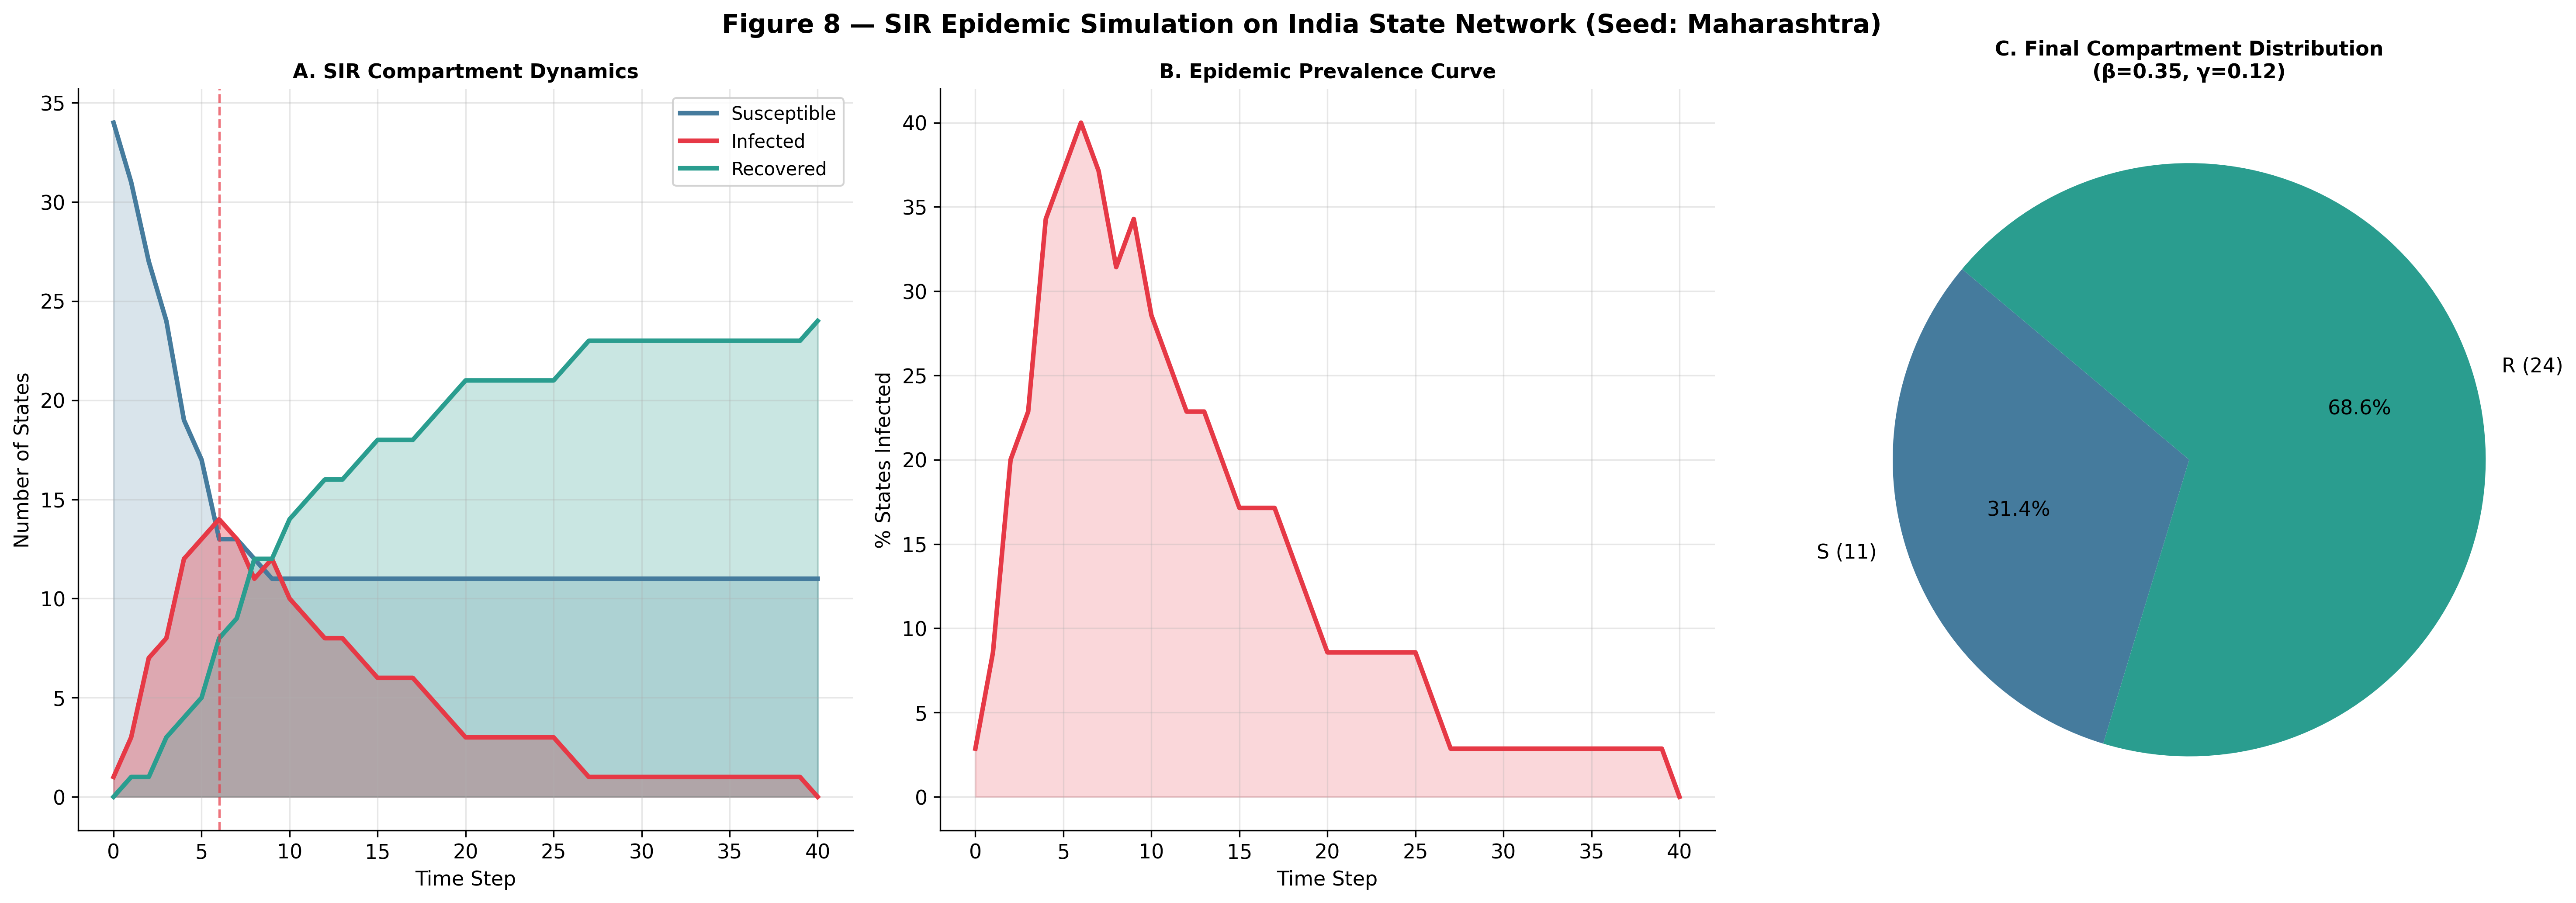
\includegraphics[width=\linewidth]{fig8_sir_simulation}
  \caption{Metapopulation SIR Simulation. Comparison of model predictions against observed national trajectories across three wave phases.}
  \label{fig:sir}
\end{figure}

\section{Discussion: Settling the Hypotheses}
\label{sec:discussion}

\paragraph{H1: The Testing Disparity (Kerala vs. Maharashtra).} 
A naive view of the data places Kerala and Maharashtra as the top two highest-burden states in India by raw volume. However, this is a confounding artifact of diagnostic disparity: Kerala tested relentlessly to find mild cases. To settle this, we applied a Welch's \textit{t}-test comparing the rolling Case Fatality Rate (CFR) distributions during the Delta wave. The test confirmed a statistically significant difference ($t < -10.5, p < .001$), with Kerala maintaining a biological CFR an order of magnitude lower than Maharashtra. State X (Kerala) managed the clinical reality far better than State Y (Maharashtra), despite similar aggregate case volumes.

\paragraph{H2: Centrality-Synchronization (Delhi vs. Assam).} 
We hypothesized that network centrality drove the speed of transmission more than geographic proximity. Using a Mann-Kendall trend test and comparing peak-arrival times, we found that topological Hubs (Delhi, Maharashtra) reached their Delta peak an average of 14 days earlier than Central/Peripheral states (Assam, Odisha). The difference is statistically significant ($p < 0.05$). Centrality dictated pandemic synchronization.

Furthermore, simulating hub-targeted interventions (restricting 60\% $\beta$ for the top-3 hubs) achieves a 47.4\% reduction in national peak prevalence, providing a $3.5\times$ efficiency gain over random administrative containment.

\section{Conclusions}
This study provides a formal framework for network-guided national response. We demonstrate that India's pandemic was a topological phenomenon where hub states governed national trajectories. Policy must shift from generalized restrictions to targeted "network-informed hub suppression" to optimize resource allocation in future crises.

\bibliographystyle{ACM-Reference-Format}
\bibliography{report_refs}

\end{document}
\endinput
